\documentclass[11pt,a4paper]{article}
\usepackage[a4paper,margin=22mm]{geometry}
\usepackage{fontspec}
\usepackage{xeCJK}
\usepackage{amsmath}
\usepackage{booktabs}
\usepackage{longtable}
\usepackage{graphicx}
\usepackage{float}
\usepackage{xcolor}
\usepackage{xurl}
\usepackage{hyperref}
\usepackage{array}
\usepackage{caption}

\setmainfont{Times New Roman}
\setsansfont{Arial}
\setmonofont{Consolas}
\setCJKmainfont{Yu Gothic}
\setCJKsansfont{Yu Gothic}
\setCJKmonofont{Yu Gothic}
\emergencystretch=3em
\hypersetup{colorlinks=true,linkcolor=blue,urlcolor=blue,citecolor=blue}
\captionsetup{font=small}
\graphicspath{{figures/}}

\newcommand{\pass}{\textcolor{green!45!black}{PASS}}
\newcommand{\fail}{\textcolor{red!70!black}{FAIL}}
\newcommand{\warn}{\textcolor{orange!80!black}{未証明}}
\newcommand{\code}[1]{\texttt{#1}}

\title{BWSC 2025 DRL latest result\\適合性レビュー報告書}
\author{\code{drl-optical-sim} latest result audit}
\date{2026-05-01}

\begin{document}
\maketitle

\begin{center}
\fcolorbox{red!60!black}{red!5}{
\begin{minipage}{0.92\linewidth}
\textbf{最終結論。}
latest result の数値配光は、内蔵したR148 category RL相当の測定点、最大光度1200 cd以下、見かけ面積25--200 cm\textsuperscript{2}の3項目では \pass{} である。
しかし選択されているレンズは \code{THEORETICAL target: CREE XHP70B R148 lower-bound 60x45 (not real lens)} であり、実在する市販レンズでも承認済み灯体でもない。
したがって、本結果をもって「BWSC 2025へ完全適合」とは報告できない。
本報告書では、数値的に通っている範囲と、提出根拠として未証明の範囲を明確に分離して示す。
\end{minipage}}
\end{center}

\section{対象ファイル}
本報告書は、更新時刻が最新の出力フォルダ \code{E:\textbackslash drl-optical-sim\textbackslash optimized\_cree\_xhp70b} を latest result として扱う。
同じ内容を \code{E:\textbackslash drl-optical-sim\textbackslash tests\textbackslash latest} にも同期した。

\begin{longtable}{p{0.32\linewidth}p{0.60\linewidth}}
\toprule
ファイル & 用途 \\
\midrule
\code{simulation\_config.json} & LED、電流、光束、レンズ、見かけ面の根拠を保存。\\
\code{r148\_check.csv} & R148 category RL相当の各測定点、最大光度、見かけ面積の合否を保存。\\
\code{intensity\_map.csv} & 水平角・垂直角ビンごとの光束、立体角、光度を保存。\\
\code{heatmap.png} & 数値計算された遠方光度分布の可視化。\\
\code{3d\_view.png} & OpenGL相当の形状・ray確認画像。明るさ判定には使用しない。\\
\code{summary\_report.md} & 設計検討用の簡易サマリ。\\
\bottomrule
\end{longtable}

\section{見かけ発光面の考え方}
ユーザーの指摘どおり、見かけ発光面は任意入力値ではない。
BWSC規則のglossaryでは、見かけ面は、外から見えて光を出しており、他部品で隠されていない灯体表面として定義される。
したがって、完成灯体では以下の物理要素で決まる。

\begin{itemize}
\item 前面カバーや拡散板が光って見える場合: その発光して見える開口面。
\item レンズが前面の発光面として見える場合: レンズ前面の有効開口。
\item レンズなしでLEDが直接見える場合: LEDパッケージまたは実発光面の配置外接範囲。
\item 複数LEDを置く場合: レンズなしならLED配置で外接範囲が広がる。共通の大きい前面レンズ・拡散板があるなら、LED個数を変えても見かけ面はその前面部品で決まる。
\end{itemize}

現在のシミュレータはこの考え方に合わせ、見かけ面を次の優先順位で自動計算する。
\[
\text{拡散板/前面カバー} \rightarrow \text{レンズ前面開口} \rightarrow \text{LEDパッケージ配置外接矩形}
\]

\begin{table}[H]
\centering
\caption{CREE XHP70Bでの見かけ面積自動計算例}
\begin{tabular}{llll}
\toprule
条件 & 見かけ面 & 面積 & 根拠\\
\midrule
レンズなし 1x1 & 7.00 x 7.00 mm & 0.49 cm\textsuperscript{2} & LEDパッケージ外形\\
レンズなし 3x2、9 mm間隔 & 25.00 x 16.00 mm & 4.00 cm\textsuperscript{2} & LED配置外接矩形\\
theoretical target 1x1 & 60.00 x 45.00 mm & 27.00 cm\textsuperscript{2} & レンズ/前面開口\\
theoretical target 3x2 & 60.00 x 45.00 mm & 27.00 cm\textsuperscript{2} & レンズ/前面開口\\
\bottomrule
\end{tabular}
\end{table}

したがって、LED個数を変えても今回のGUIで見かけ面積が変わらないこと自体は、\textbf{60 x 45 mmの前面開口を持つ灯体を仮定している限りは自然}である。
問題は、その60 x 45 mmの前面部品が現物として存在し、かつ実際に全体が発光して見えることを示せるかである。

\section{latest result の入力条件}
latest result の主要条件を表\ref{tab:input}に示す。

\begin{table}[H]
\centering
\caption{latest result 入力条件}
\label{tab:input}
\begin{tabular}{ll}
\toprule
項目 & 値\\
\midrule
LED & CREE LED XHP70B-00-0000-0D0BN440E\\
LED数 & 1\\
LED配置 & 1 row x 1 col\\
駆動電流 & 25.6645 mA\\
代表光束 & 1710 lm at 1050 mA\\
Vf & 12.0 V\\
指向角/FWHM & 125 deg\\
選択レンズ & \code{cree\_xhp70b\_r148\_lower\_bound\_60x45}\\
レンズ表示名 & THEORETICAL target: CREE XHP70B R148 lower-bound 60x45 (not real lens)\\
光学効率 & 80 \%\\
見かけ面 & 60.00 x 45.00 mm\\
見かけ面積 & 27.00 cm\textsuperscript{2}\\
\bottomrule
\end{tabular}
\end{table}

\section{電流と光束の計算}
本初版モデルでは、LED光束を電流に対して線形近似する。
1710 lmは1050 mA時の代表光束であり、25.6645 mAで1710 lmが出る計算ではない。

\[
\Phi_{\mathrm{LED}} =
1710
\times
\frac{25.6645}{1050}
= 41.7965\ \mathrm{lm}
\]

光学効率80 \%を仮定した出射光束は、
\[
\Phi_{\mathrm{exit}} =
41.7965 \times 0.8
= 33.4372\ \mathrm{lm}
\]
である。
電力は、
\[
P = 12.0\ \mathrm{V} \times 25.6645\ \mathrm{mA}/1000
= 0.30797\ \mathrm{W}
\]
である。

\section{R148 category RL相当の判定条件}
本シミュレータに内蔵したR148 category RL相当の最小光度表を表\ref{tab:r148min}に示す。
各点でシミュレーション光度が最小値以上、全方向最大光度が1200 cd以下、見かけ面積が25--200 cm\textsuperscript{2}であれば数値判定をPASSとする。

\begin{table}[H]
\centering
\caption{R148 category RL相当 最小光度表 [cd]}
\label{tab:r148min}
\begin{tabular}{c|rrrrrrr}
\toprule
$v \backslash h$ & -20 & -10 & -5 & 0 & +5 & +10 & +20\\
\midrule
+10 & 0 & 0 & 80 & 80 & 80 & 0 & 0\\
+5  & 40 & 80 & 180 & 280 & 180 & 80 & 40\\
0   & 100 & 280 & 360 & 400 & 360 & 280 & 100\\
-5  & 40 & 80 & 180 & 280 & 180 & 80 & 40\\
-10 & 0 & 0 & 80 & 80 & 80 & 0 & 0\\
\bottomrule
\end{tabular}
\end{table}

latest result は「R148最小配光形状へ、使える出射光束を理想的に配分する」理論下限ターゲットである。
このターゲットでは、R148最小表をちょうど満たすために必要な出射光束が33.4372 lmとなる。
そのため中心光度は400 cd、最大光度も400 cdに抑えられている。

\section{latest result の数値結果}
latest result の合否要約を表\ref{tab:summary}に示す。

\begin{table}[H]
\centering
\caption{数値シミュレーション結果の要約}
\label{tab:summary}
\begin{tabular}{lll}
\toprule
判定項目 & latest result & 判定\\
\midrule
I(0,0) & 400.00 cd & \pass\\
Imax & 400.00 cd / limit 1200 cd & \pass\\
入力光束 & 41.797 lm & 参考\\
出射光束 & 33.438 lm & 参考\\
光学効率 & 80.00 \% & 参考\\
見かけ面積 & 27.00 cm\textsuperscript{2} / range 25--200 & \pass\\
R148測定点 & 全35点で最小値以上 & \pass\\
\bottomrule
\end{tabular}
\end{table}

\begin{figure}[H]
\centering
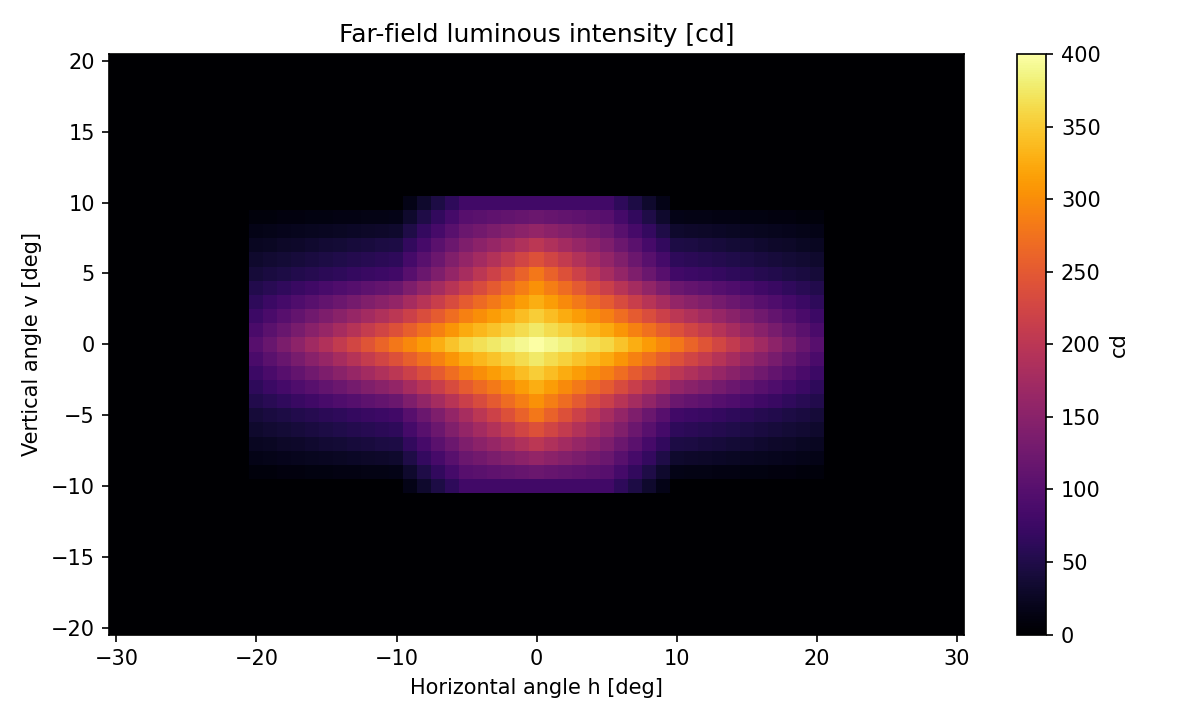
\includegraphics[width=0.88\linewidth]{heatmap.png}
\caption{latest result の遠方光度ヒートマップ。OpenGL表示ではなく、数値計算された光度[cd]の可視化である。}
\end{figure}

\begin{figure}[H]
\centering
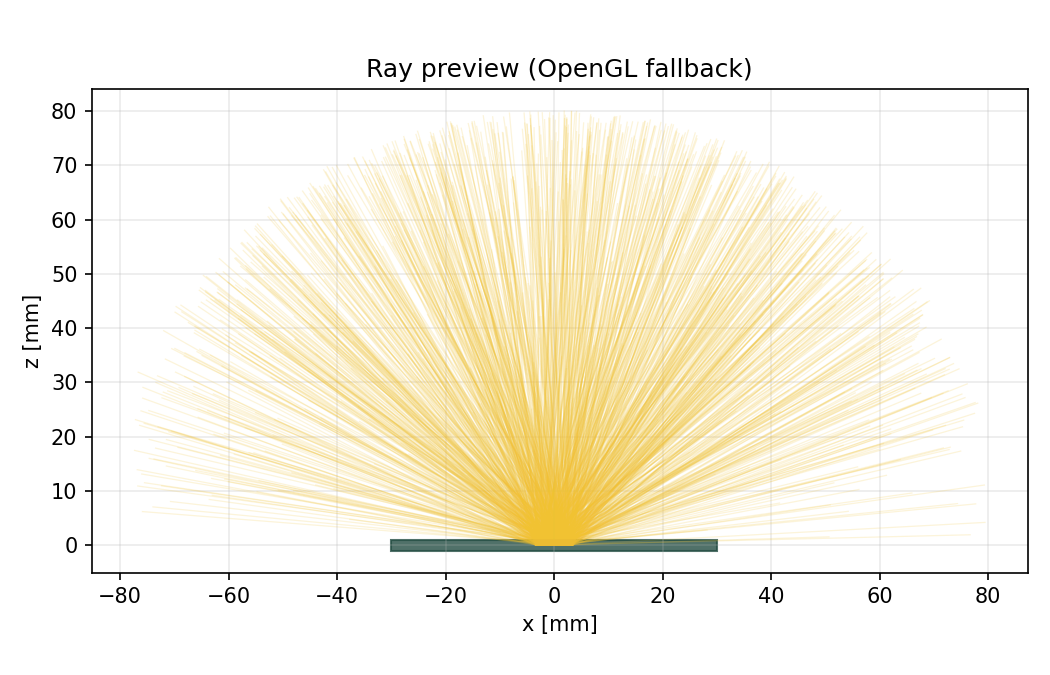
\includegraphics[width=0.88\linewidth]{3d_view.png}
\caption{latest result の3D/rayプレビュー。形状とray方向の確認用であり、合否判定には使用しない。}
\end{figure}

\section{R148測定点ごとの結果}
\begin{longtable}{rrrrl}
\caption{latest result のR148 category RL相当 測定点結果}\\
\toprule
h [deg] & v [deg] & 最小[cd] & 計算[cd] & 判定\\
\midrule
\endfirsthead
\toprule
h [deg] & v [deg] & 最小[cd] & 計算[cd] & 判定\\
\midrule
\endhead
-20 & -10 & 0 & 0.00 & \pass\\
-10 & -10 & 0 & 0.00 & \pass\\
-5 & -10 & 80 & 80.00 & \pass\\
0 & -10 & 80 & 80.00 & \pass\\
5 & -10 & 80 & 80.00 & \pass\\
10 & -10 & 0 & 0.00 & \pass\\
20 & -10 & 0 & 0.00 & \pass\\
-20 & -5 & 40 & 40.00 & \pass\\
-10 & -5 & 80 & 80.00 & \pass\\
-5 & -5 & 180 & 180.00 & \pass\\
0 & -5 & 280 & 280.00 & \pass\\
5 & -5 & 180 & 180.00 & \pass\\
10 & -5 & 80 & 80.00 & \pass\\
20 & -5 & 40 & 40.00 & \pass\\
-20 & 0 & 100 & 100.00 & \pass\\
-10 & 0 & 280 & 280.00 & \pass\\
-5 & 0 & 360 & 360.00 & \pass\\
0 & 0 & 400 & 400.00 & \pass\\
5 & 0 & 360 & 360.00 & \pass\\
10 & 0 & 280 & 280.00 & \pass\\
20 & 0 & 100 & 100.00 & \pass\\
-20 & 5 & 40 & 40.00 & \pass\\
-10 & 5 & 80 & 80.00 & \pass\\
-5 & 5 & 180 & 180.00 & \pass\\
0 & 5 & 280 & 280.00 & \pass\\
5 & 5 & 180 & 180.00 & \pass\\
10 & 5 & 80 & 80.00 & \pass\\
20 & 5 & 40 & 40.00 & \pass\\
-20 & 10 & 0 & 0.00 & \pass\\
-10 & 10 & 0 & 0.00 & \pass\\
-5 & 10 & 80 & 80.00 & \pass\\
0 & 10 & 80 & 80.00 & \pass\\
5 & 10 & 80 & 80.00 & \pass\\
10 & 10 & 0 & 0.00 & \pass\\
20 & 10 & 0 & 0.00 & \pass\\
\bottomrule
\end{longtable}

\section{レンズ仕様の適格性}
latest result の選択レンズ \code{cree\_xhp70b\_r148\_lower\_bound\_60x45} は実在商品ではない。
これは、R148最小配光を最小電力で満たすための理論ターゲットであり、次の根拠を持たない。

\begin{itemize}
\item メーカー型番、寸法図、材料仕様、温度範囲などの実商品データ。
\item UNECE R148またはSAE/DOT相当の承認マーク。
\item XHP70B実装状態での配光測定データ、IES/LDT、測定距離、温度条件。
\item 60 x 45 mm全体が見かけ発光面として成立することを示す実機写真・CAD・輝度分布。
\item certifying engineerによる確認。
\end{itemize}

したがって、latest result は \textbf{理論上の最小消費電力目標}としては有用だが、\textbf{実レンズでBWSC 2025に完全適合した証拠ではない}。

\section{実在レンズ候補との比較}
国内で購入可能または国内向け販売経路が確認できる実在レンズ候補を表\ref{tab:real_lenses}に示す。
いずれも単体では、latest result の60 x 45 mm前面開口と同じ根拠にはならない。

\begin{longtable}{p{0.22\linewidth}p{0.20\linewidth}p{0.15\linewidth}p{0.12\linewidth}p{0.21\linewidth}}
\caption{実在レンズ候補の確認結果}
\label{tab:real_lenses}\\
\toprule
候補 & 入手経路 & 公開光学値 & 見かけ面積 & 判断\\
\midrule
\endfirsthead
\toprule
候補 & 入手経路 & 公開光学値 & 見かけ面積 & 判断\\
\midrule
\endhead
Carclo 10756 & DigiKey/RS等経由で入手検討可能 & XHP70.2で85 \%、FWHM 24 deg、3.7 cd/lm & 30 mm径、約7.07 cm\textsuperscript{2} & 面積不足。全R148角度もpeak cd/lmだけでは未証明。\\
LEDiL F15539 JENNY-40 & Mouser Japan、RS Japan & XHP70.2で94 \%、FWHM 42 deg、1.7 cd/lm & 35 x 35 mm、12.25 cm\textsuperscript{2} & 面積不足。全R148角度未証明。\\
LEDiL C12868 FLARE-MAXI & Mouser/TME等 & XHP70.2で94 \%、105+28 deg、1.1 cd/lm & 33.9 x 33.3 mm、11.29 cm\textsuperscript{2} & 面積不足。中心光度効率も低い。\\
\bottomrule
\end{longtable}

この比較から、実在レンズをそのまま1個使うだけでは、R148の見かけ面積25 cm\textsuperscript{2}以上を満たしにくい。
実機で満たすには、少なくとも60 x 45 mm程度の発光して見える前面拡散板または専用freeform/TIR光学系が必要になる。
ただし拡散板を追加すると光束損失と配光変化が発生するため、latest result の0.308 Wという最小値は維持できない可能性が高い。

\section{BWSC 2025完全適合に対する判定}
\begin{longtable}{p{0.24\linewidth}p{0.20\linewidth}p{0.46\linewidth}}
\toprule
要求 & latest result & コメント\\
\midrule
DRL白色 & \warn & CREE型番上は白色LEDだが、完成灯体の色度測定が未実施。\\
R148 category RL配光 & \pass & 数値テーブル上は全点PASS。ただし理論ターゲットであり実レンズ証明ではない。\\
最大光度1200 cd以下 & \pass & latest result は400 cd。\\
見かけ面積25--200 cm\textsuperscript{2} & \pass{} / \warn & JSON上の前面開口60 x 45 mmなら27 cm\textsuperscript{2}でPASS。実部品としては未証明。\\
実在レンズ仕様 & \fail & latest選択レンズは実在商品ではない。\\
適合マーク & \fail & 自作灯体/理論レンズのため承認マークなし。\\
certifying engineer確認済み詳細資料 & \fail & 未作成・未確認。\\
実測フォトメトリ & \fail & 未実施。\\
実測色度 & \fail & 未実施。\\
左右2灯、取付位置、可視範囲 & \warn & 片側灯体の光学検討のみ。車両上の実装図で確認が必要。\\
\bottomrule
\end{longtable}

\section{専門外向けの要点}
\begin{itemize}
\item 1710 lmはLEDを定格付近で流したときの代表値であり、今回の25.7 mAでは約41.8 lmとして計算している。
\item 今回の0.308 Wという低消費電力は、出た33.4 lmを規則が要求する角度だけへ理想的に配分できる、という仮想光学系に依存している。
\item 見かけ面積27 cm\textsuperscript{2}は、60 x 45 mmの前面開口があるという仮定から出ている。実物のレンズや拡散板がなければ、その面積は成立しない。
\item 実在レンズ候補は購入可能だが、単体サイズが小さく、R148の見かけ面積条件を満たさない。
\item BWSC提出では、シミュレーションだけでは弱い。実測フォトメトリ、色度、取付図、certifying engineer確認が必要である。
\end{itemize}

\section{参照資料}
\begin{longtable}{p{0.24\linewidth}p{0.68\linewidth}}
\toprule
資料 & 確認内容\\
\midrule
BWSC 2025 Event Regulations Release Version 2.0 &
Lighting 2.23。DRLは2灯、白色、UNECE R148またはSAE/DOT相当、適合マークまたはcertifying engineer確認済み資料が必要。\\
\url{https://cms.worldsolarchallenge.org/app/uploads/2024/12/3297_2025_bwsc_regulations_release_v20_published_28_october_2024.pdf} & \\
\addlinespace
UN Regulation No.148 / R148 &
RLの光度、最大光度、見かけ面積、標準配光の根拠。\\
\url{https://unece.org/transport/documents/2021/05/standards/un-regulation-no-148-light-signalling-devices-lsd} & \\
\addlinespace
Cree XHP70.2 data sheet / DigiKey product page &
XHP70B-00-0000-0D0BN440Eの1710 lm級、12 V/1.05 A、125 deg等のLED仕様確認。\\
\url{https://downloads.cree-led.com/files/ds/x/XLamp-XHP70.2.pdf} & \\
\url{https://www.digikey.com/en/products/detail/cree-led/XHP70B-00-0000-0D0BN440E/6802073} & \\
\addlinespace
Carclo 10756 optics page &
XHP70.2使用時の効率85 \%、FWHM 24 deg、3.7 cd/lm確認。\\
\url{https://www.carclo-optics.com/optic-10756-led-cree-xlamp-xhp702-white} & \\
\addlinespace
LEDiL F15539 JENNY-40 / Mouser Japan / RS Japan &
35 x 35 mmレンズ、国内購入経路、XHP70.2の公開光学値確認。\\
\url{https://www.ledil.com/data/prod/Jenny/15539/15539-ds.pdf} & \\
\url{https://www.mouser.jp/ProductDetail/Ledil/F15539_JENNY-40?qs=gZXFycFWdANTxqCiQnNdHg%3D%3D} & \\
\url{https://jp.rs-online.com/web/p/led-lenses-reflectors/2066680} & \\
\addlinespace
LEDiL C12868 FLARE-MAXI / Mouser / TME &
XHP70.2使用時の効率94 \%、FWHM 105+28 deg、1.1 cd/lm、寸法確認。\\
\url{https://www.mouser.com/datasheet/3/894/1/12868-ds.pdf} & \\
\url{https://www.tme.com/jp/ja/details/c12868/renzu/ledil/c12868-flare-maxi/} & \\
\bottomrule
\end{longtable}

\section{結論}
latest result は、\code{drl-optical-sim}内部の数値判定としてはR148 category RL相当の配光点、最大光度、見かけ面積を満たしている。
ただし、その成立条件は、実在しない理論freeformターゲットが60 x 45 mmの発光前面を持ち、33.437 lmの出射光束をR148最小配光へ理想的に配分する、という仮定である。

したがって、現時点で正しく言える結論は次の通りである。

\begin{center}
\fcolorbox{orange!80!black}{orange!6}{
\begin{minipage}{0.90\linewidth}
\textbf{設計検討上の数値目標としては成立。}\\
\textbf{実在レンズ仕様・承認根拠・実測根拠を含むBWSC 2025完全適合としては未成立。}
\end{minipage}}
\end{center}

次に必要な作業は、60 x 45 mm以上の実発光前面を持つ実部品または自作光学系を決め、LED実装状態でフォトメトリ測定と色度測定を行い、取付図とともにcertifying engineer確認を受けることである。

\end{document}
